In this chapter, our framework will be evaluated using a variation of the Goal-QuestionMetric (GQM) technique \cite{van2002goal}. The GQM plan has been slightly modified by the addition of a new column with the results. The questions pertinent to evaluating our strategy and its outcomes are separated into two primary sections: the first related to the algorithm utilized in the pattern analysis process itself, and the other about the method's overall efficacy. Table \ref{tab:gqm_plan} details the study questions.

\begin{table}[!h]
    \centering
    \begin{tabular}{ccl}
    \hline
    \multicolumn{3}{|c|}{\textbf{Goal 1}: Property Violation Identification process}                                                                                                                            \\ \hline
    \multicolumn{1}{|c|}{Question}                                                                                    & \multicolumn{1}{c|}{Metric}                     & \multicolumn{1}{c|}{Results} \\ \hline
    \multicolumn{1}{|c|}{\makecell{How well does our model \\ generalize to unseen data?}}                                         & \multicolumn{1}{c|}{\makecell{Precision and \\Recall Rates}} & \multicolumn{1}{c|}{\makecell{Precision: 1.0 \\ Recall: 0.9958}}        \\ \hline
                                                                                                                      &                                                 &                              \\ \hline
    \multicolumn{3}{|c|}{\textbf{Goal 2}: Method's contribuition}                                                                                                                                               \\ \hline
    \multicolumn{1}{|c|}{Question}                                                                                    & \multicolumn{1}{c|}{Metric}                     & \multicolumn{1}{c|}{Results} \\ \hline
    \multicolumn{1}{|c|}{\makecell{How effective is our approach \\ in the discovery of patterns \\in property violation scenarios?}} & \multicolumn{1}{c|}{\makecell{Number of \\patterns found}}   & \multicolumn{1}{c|}{\makecell{49 patterns \\11 Groups}}        \\ \hline
    \end{tabular}
    \caption{GQM Plan}
    \label{tab:gqm_plan}
\end{table}

\section{Experimental Setup}

The evaluation of our proposed solution will rely on a implementation of the Body Sensor Network described in Section \ref{BSN}. Our version of this CPS includes a Central Node and five sensors: an oximeter, a thermometer, a heart rate monitor, and an APBD and APBS blood pressure sensors. The patient's readings are assessed within each sensor node, where the health risk percentage of the monitored vital sign is calculated. Subsequently, the risk percentage is relayed to the Central Node, which, in turn, is in charge of collecting and fusing the data from the sensors, assessing the patient's overall risk, and indicating an emergency if one is discovered.

\subsection{Innate Immunity through Assurances}

\subsubsection{Prototype Implementation}

\begin{figure}[!h]
	\centering
	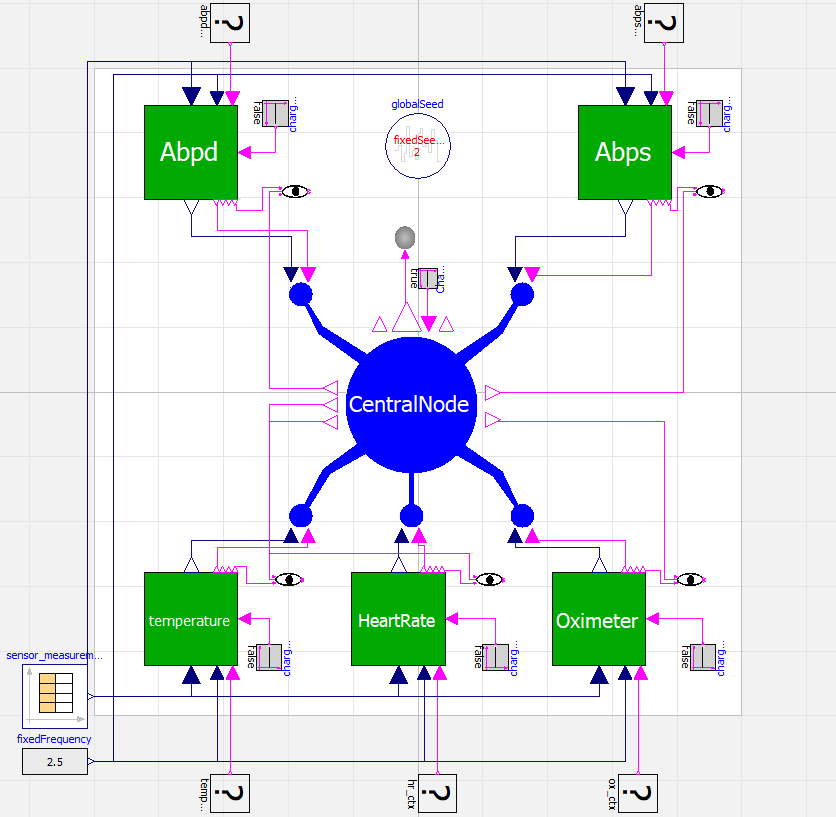
\includegraphics[width=0.7\textwidth, keepaspectratio]{img/BSN_prototype_Modelica.png}
	\caption{BSN Prototype Implemented in OpenModelica}
	\label{fig:BsnProt}
\end{figure}

The first part of our technique requires the implementation of a CPS prototype. This is done to anticipate problems that may occur during runtime by modeling and simulating both the system's software components and physical processes. Despite the fact that there are several state-of-the-art approaches for designing such models \cite{baras2019formal} \cite{deng2019modeling} \cite{bouskela2022formal}, and since the focus of this work is to elaborate on the property violation patterns using the NSA, a simpler framewrok for the simulation was selected. The Modelica language \cite{Modelica}, hence, will be used as the main tool in this process. This language is powerfull enough to represent the acausal continuous-time physical processes of the CPS through equations. It also comprises several built-in libraries for the modeling of circuits, batteries, fluids, noise, equipment deterioration and so on. At the same time, software components can also be described by defining algorithms and functions that account for the behavior of such modules. The graphical aid is achieved by the OpenModelica \cite{OpenModelica} modeling tool, in which the components and their interactions can be visually modeled as blocks and connectors.


Figure \ref{fig:BsnProt} depicts the prototype that was implemented in OpenModelica, using the Modelica language. The green blocks account for the sensors, while the blue illustrates the Central Node. In the left lower side, a parameter defines a fixed frequency for data collection that is utilized by every sensor, and above it there is a reference for an external csv file that contains the measurements of the sensors at every second. Around the system, there are some blocks with question marks whose function is to generate random binary numbers to indicate whether the sensor was active. The goal of these blocks is to simulate cases when the sensor stopped responding, or was too far away to transmit reliable data, or had some malfunctioning of sorts that may account for faults in runtime. Next to the sensors there are some gray boxes that are used to indicate when the sensor is plugged into the outlet. Besides that, there are also small rounded blocks that represent the observers, that are modeled to monitor properties of the system associated with each sensor.

\begin{figure}[!h]
	\centering
	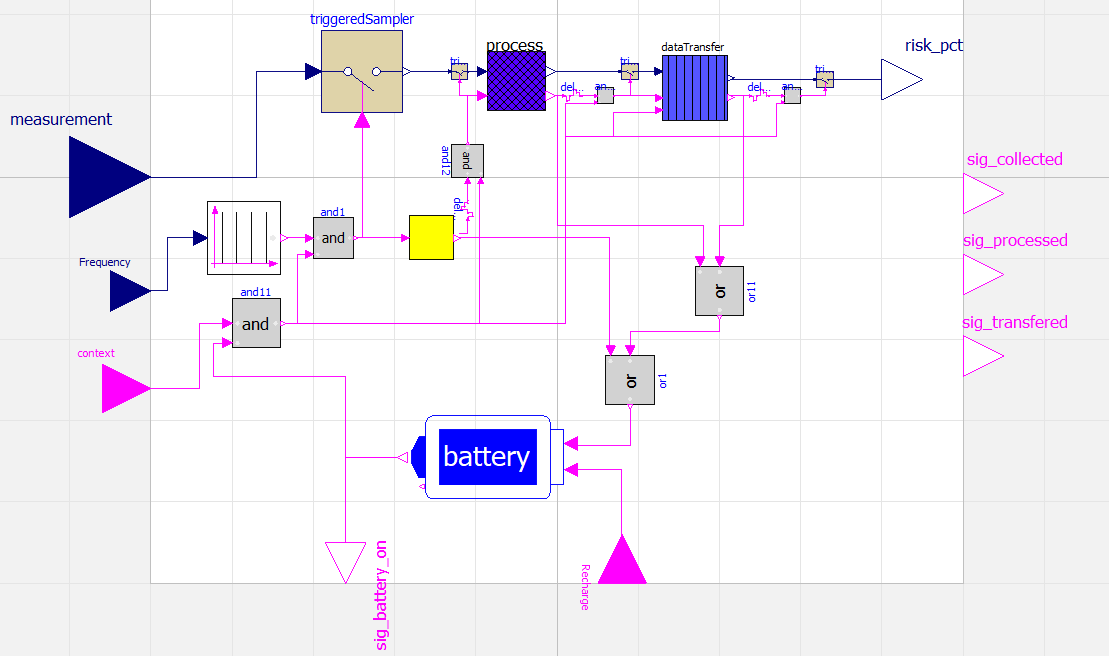
\includegraphics[width=0.7\textwidth, keepaspectratio]{img/sensor_modelica.png}
	\caption{The model of a sensor implemented in OpenModelica}
	\label{fig:sensorProt}
\end{figure}

By going one step deeper into the model, it is possible to describe how the inner workings of the sensors and the Central Node were implemented. One of the advantages of the Modelica language is its object-oriented character that allows for the reuse of modules throughout the simulation. The sensor described in Figure \ref{fig:sensorProt} is a good example of this aspect, since the same block is used to model all five sensors. The physical components represented here comprise: a mechanism for sampling a measurement based on a triggered signal, a set of bitwise operators that are often used in microcontroller programming, and a battery. This battery was modeled based on a built-in Modelica library that allows for the modeling of electric circuits, and is composed of a set of switches, a memory cell, and a signal current converter that receives signals from the sensor whenever some process occur to decrease the charge of the memory cell. The magnitude of the charge decrease is multiplied by a randomly generated real number in a way that simulates the decrease that would happen in a real environment. Meanwhile, software components of the sensor are also modeled, like the Process block, which recieves a real valued sensor measurement as an input and relies on an algorithm for determining the health risk percentage of the patient.


The Central Node, illustrated in Figure \ref{fig:centralNodeProt}, was implemented in a similar fashion. It also makes use of bitwise operations for handling the signals sent, and of an instance of the same battery model as the one found in the sensors. The software components encapsulate functions that fuse the data from the sensors and compute the overall health risk of the patient.

\begin{figure}[!h]
	\centering
	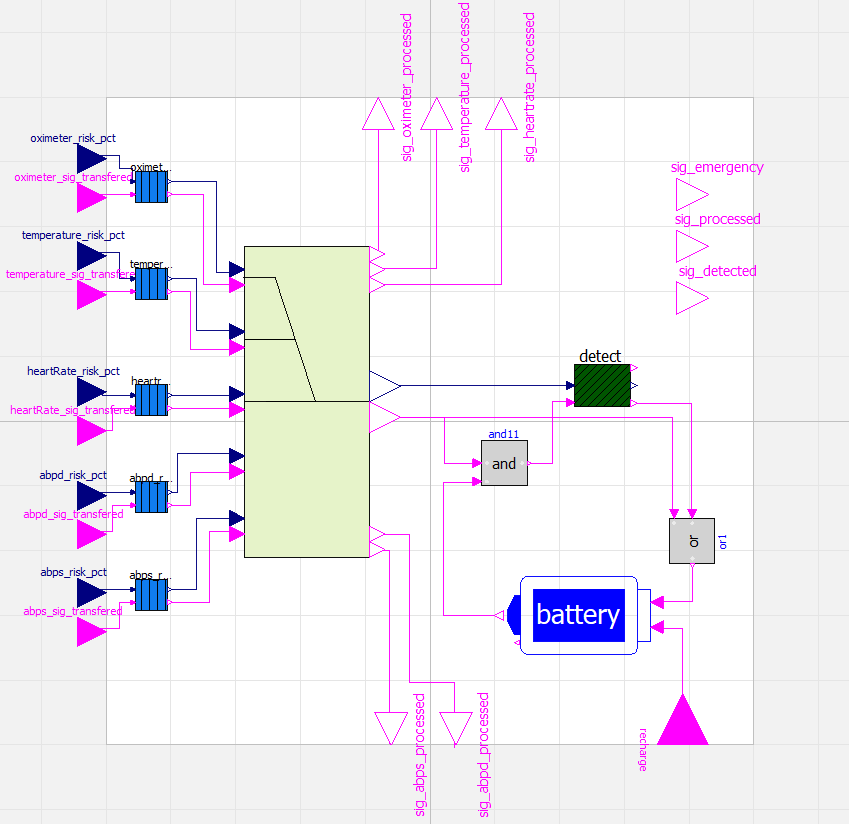
\includegraphics[width=0.7\textwidth, keepaspectratio]{img/central_node_modelica.png}
	\caption{The model of the Central Node implemented in OpenModelica}
	\label{fig:centralNodeProt}
\end{figure}

Both the sensors and the Central Node are instrumented through a set of signals that are sent each time a process or a specfic behavior occur, like when the data is collected or transfered for instance. These signals are used by the observers to monitor the properties of interest, and will be used later for the characterization of a execution segment, during the pattern analysis phase. Observers can be easily modeled in Modelica via a built-in library developed for the desing of state graphs. Both the states of the automata and its transitions are described as blocks, with the difference being that the transitions receive signals as input to indicate the passing through the states. 

Without loss of generality, to meet the proposed goals of the GQM plan, it will suffice to evaluate the accuracy and efficiency of our technique based on the analysis of a single property. Therefore, Property \textbf{P7}, from Section \ref{sec:BSN} was chosen to guide the next phase of the methodology, since it is related to all the different modules of the CPS. The property states as follows: "Whenever a sensor node has collected data, in within at most 2 seconds, the Central Node will process it." It focuses on the reliability of the system, since its satisfaction guarantees that the collected data will be processed in a reasonable time. Besides that, the Oximeter was the sensor chosen to reify the analysis. 

With that being said, the observer related to \textbf{P7}, implemented in the work of Carwehl et al. \cite{2022PSP}, will be deployed in this simulation. The states of the automata were modeled as blocks and the transitions as instances of the \textit{TransitionWithSignal} class of the StateGraph library of Modelica. The signals used in the transitions are provided by the sensor and the Central Node, while a timer is set every time the monitor enters the CollectedReached state  and if it does not transition back to the initial state, by the time when the timer runs out, the error state is reached. 

% With that being said, the observer associated to \textbf{P7}, as implemented in the work of Carwehl et al. \cite{2022PSP}, was used in this simulation. The automata's states were represented as blocks, and the transitions as instances of the \textit{TransitionWithSignal} class from Modelica's StateGraph package. The sensor and the Central Node provide the signals utilized in the state transitions, while a timer is started every time the monitor reaches the CollectedReached state, and if it does not transition back to the starting state when the timer runs out, the error state is reached.


\begin{figure}[!h]
	\centering
	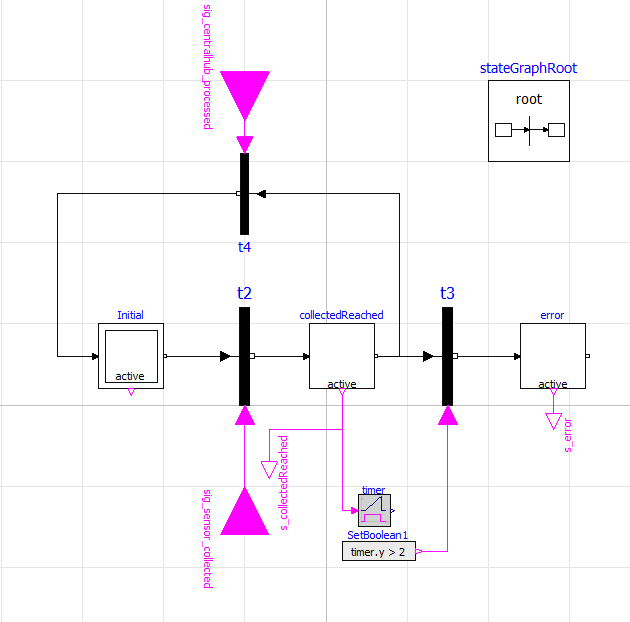
\includegraphics[width=0.7\textwidth, keepaspectratio]{img/obs_modelica.png}
	\caption{The model of the Observer implemented in OpenModelica}
	\label{fig:obsProt}
\end{figure}

\subsubsection{Prototype Simulation}

With the prototype of the BSN in place, several simulations were executed with varying configurations, patient profiles and environment variables so that the complexities of runtime could be assessed earlier. 

As noted in the preceding section, one of the simulation's inputs is a csv file holding the sensors' readings at each second. The patient profile given by these files is constructed using a randomized approach in the Python language in order to be as neutral as feasible. Three functions for generating random points within a range were created: one for indicating a rising tendency, another for indicating a decreasing tendency, and a third for keeping the data trend steady. Initially, a random point is created within the sensor's range of data. Then, one of the three functions and a second value that accounts for the "destination" are randomly picked. The function is then run for the generation of data points starting from the initial value and ending in the destination value, with the selected tendency. For large datasets, the process can be repeated with the destination value becoming the initial value of the new cycle. For example, suppose we are generating the data for the thermometer. The initial value is 36.5C, the destination value generated is 38C and the selected function is the rising tendency. Then a set of datapoints will be randomly genereated in a way that it starts from the initial value and rises until reaching 38C. This process was performed for each of the five sensors and repeated until the desired data set size.

After the creation of the dataset, the simulation was run. Even though OpenModelica makes it realy easy to perform simulations, it does not scale well, since the csv files and the system configurations must be set manually at each run. To address this problem, a python library named OMPython was used \cite{OMPython}. It is a Python-based interactive session handler for Modelica scripting that is free, open source, and extremely portable. It was utilized to programatically load the modules, alter the parameters and configurations and run the simulation.

To account for as much variability as possible, 1,000 patient profiles were randomly generated and, the same amount of simulations were performed. The operation dataset of each run was extracted and saved as csv files. The simulation was processed in an Intel(R) Core(TM) i5-10210U, 2.10 GHz, 16GB.

\subsection{Adaptive Immunity Through Learning}

After the simulations were run, the extraction of the operation dataset triggered the next phase of the methodology. Tightly related to the adaptive immune response of the BIS, the data was processed and inputed into the Negative Selection algorithm to allow for a more specific response in face of anomalous behavior.

\subsubsection{Feature engineering}

Initially, a data pipeline was built in the Python language for the processing of the operation dataset. The data was divided into execution segments based on the time constraints of the property \textbf{P7} using the procedure outlined in Section \ref{sec:feat_eng}. The segments were then summarized into single rows using domain knowledge, and features were extracted from the segment to better characterize it. For example, we created boolean features based on the signals sent between the modules of the system, which may indicate that the data was properly transfered to the Central Node, or that the sensor ceased operating during the computation of the health risk percentage. Other engineered features are related to the description of specific behaviors that might have happened, like the battery running out, or an emergency being detected. Finally, we have also developed real-valued features that reflect, for instance, how long it took to perform some task, or the measurement collected by the sensor.

The labeling task was performed by the development of an algorithm that mimics the behavior of the observer. The observer itself could have been used for this task, by simply looking at its state in the end of the segment. Nevertheless, the error state is a dead end since there are no transitions outside from it. This means that, if this state is reached in the middle of a simulation, all subsequent segments will be also accounted as faulty, even if the system properly handles the situation and goes back to its regular execution. Thus, some adjustments would be required in order to use the observer to pinpoint the traces where property violations happened, which could risk the correctness of the process. This tension was handled by implementing an algorithm that reads the engineered features and replicates the verification that would be performed by the observer. For example, the \textbf{P7} observer from Figure \ref{fig:obsProt} checks if the sensor collected data and if the Central Node has processed it. Since the execution segments are split based on the time restriction, if the Central Node does not execute, i.e. the boolean feature related to this behavior is set to \textit{False}, then we have found a property violation segment. 

\subsubsection{Negative Selection Algorithm}

For the NSA to be run on the operation dataset, first an Exploratory Data Analysis was performed. For that matter, a sanity check was realized to assess the quality of the data that was generated. Each feature was carefully inspected to see if any faults in the design or in the feature engineering process could be spotted. Examples included columns with an unexpected amount of missing values, wrong data types, and strange behaviors, like data being transfered without the sensor having collected it. After that, the correlation between each pair of features was computed as a means to remove any multicolinearity in the dataset. The idea behind it was that, since highly correlated features bring similar information, one of them can be discarded.

Next, a new correlation analysis took place, but this time only considering the relationship between the boolean features and the property violation label. As explained in Section \ref{sec:prop_NSA}, only the boolean variables were considered for they would compose the binary string in the Negative Selection Algorithm. The Matthews correlation coefficient (MCC) was utilized for this task \cite{chicco2020advantages} since it provides a truthfull and informative description of the relationship between two boolean features. The columns were sorted in a descending way based on the absolute value of the correlation rate, and a threshold of 0.1 was the basis for removing features that were not correlated with the label. The features based on the signals that the observer uses to identify violations, were also removed, since they were used in the making of the label. Table \ref{tab:pos_features} shows the 13 features that resulted from this process and their respective position related to the absolute value of the MCC rate. It can be noted that the last 4 features are related to other sensors and have a correlation close to 0.1, which could be easily removed. We, however, have decided to keep them to assess the performance of our model in the presence of noise in the data.


\begin{table}[!h]
    \begin{tabular}{clc}
    \hline
    Position & Feature                                                    & \makecell{MCC \\ (Absolute)} \\ \hline
    0        & Oximeter was available during the data transference        & 0.927324                          \\
    1        & Oximeter transfered data                                   & 0.923101                          \\
    2        & Oximeter was available during Central Node data processing & 0.849276                          \\
    3        & Oximeter Battery became unavailable at some point          & 0.508921                          \\
    4        & Oximeter became unavailable during trace                   & 0.462366                          \\
    5        & Oximeter battery became unavailable during data collection & 0.300302                          \\
    6        & Oximeter processed data                                    & 0.300302                          \\
    7        & Oximeter battery became unavailable during data processing & 0.296026                          \\
    8        & Oximeter became unavailable during data transference       & 0.269047                          \\
    9        & The battery of the ABPD sensor became unavailable          & 0.136670                          \\
    10       & The battery of the ABPS sensor became unavailable          & 0.133274                          \\
    11       & The battery of the Heart Rate monitor became unavailable   & 0.129930                          \\
    12       & The battery of the thermometer became unavailable          & 0.126224                          \\ \hline
    \end{tabular}
    \label{tab:pos_features}
    \caption{Selected Features and their respective positions}
\end{table}


Finally, the Negative Selection Algorithm was run, based on the simulation generated dataset and on the selected features. The training phase aims at generating the nonself detectors that will hold the patterns of the anomalous segments. First, the nonself-data, i.e. the rows labeled as property violations, were removed from the set. Then, Afterwards, the execution segments were modeled as binary strings, following the features and positions from Table \ref{tab:pos_features}. Next, while the desired number of detectors was not reached, a binary string of length \(r = 5\) would be generated and tested against the execution segment strings for matching. In the case of a match, the detector candidate would be discarded. Otherwise, it was appended in a list of nonself detectors. The matching function works as follows: for each position \(p\), with \(0 \leq p \leq 8\), the algorithm would check if there was a substring of length \(l=r=5\) in the self-set, starting in position \(p\), that was equal to the candidate detector. If the algorithm unsuccessfully attempts to generate a viable detector for a predefined number of times, then the algorithm goes through an early stop.

\section{Goal 1: Property Violation Identification process}

\textbf{Question: How well does our model generalizes to unseen data?} To answer this question propertly, the operation dataset extracted from the simulations was splitted into two: 75\% of the set was used for the detector's generation, and the other 25\% was set apart to account for the unseen data. The entire dataset had 19868 rows, with 16493 (83\%) related to regular operation and 3375 (17\%) of the execution segments violated property \textbf{P7}. Hence, the split resulted in 14901 rows being utilized in the training phase, but only 12370 rows were used for the generation of the nonself detectors, since the process only makes use of the self-set, i.e. the majority class.

\begin{figure}[!h]
	\centering
	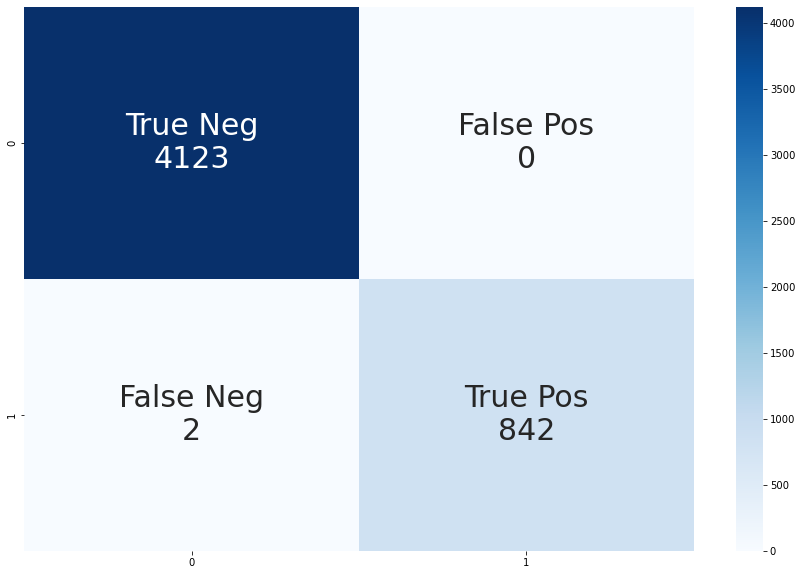
\includegraphics[width=0.5\textwidth, keepaspectratio]{img/NSA_confusion_matrix.png}
	\caption{NSA's Confusion Matrix}
	\label{fig:nsa_conf}
\end{figure}

We are using the metrics of precision and recall to assess the performance of the model, since they provide a good summary of the confusion matrix. The recall rate is computed as \textit{True Positives} / (\textit{True Positives + False Positives}), i.e. how many of the relevant property violations were found, while the precision rate is calculated as \textit{True Positives} / (\textit{True Positives + False Negatives}), and is the same as asking "how many property violations found were relevant." Our main interest was in having a high precision rate, since we wanted to have the lowest value of \textit{False positives} as possible. This happens because the goal was to study the generated detectors to understand the patterns found, and having \textit{False positives} could impact in this task. On the other hand, having \textit{False Negatives} would not have such impact, once they would be related to the patterns that were not discovered by the detectors, thus causing less harm to the overall approach. Figure \ref{fig:nsa_conf} depicts the confusion matrix of the results of the model. No self-data was considered as faulty, meaning that there were no \textit{False Positives}, as desired. Nevertheless, only 2 violations were not assessed by the NSA, which is within an acceptable range.


Table \ref{tab:ev_comparison} shows the precision and recall rates of our approach using the Negative Selection Algorithm over the simulation dataset in relation to the property \textbf{P7} for the Oximeter sensor. The accuracy and MCC rates were also computed as a way to have a complementary view on the performance. Besides that, the same labeled dataset was also used as input for some well known Machine Learning algorithms. The One-class SVM and the Isolation Forest were brought to this comparison since they are algorithms utilized in anomaly detection tasks, and because the One-class SVM is usually compared with the NSA for they both use only one of the classes during the training phase \cite{NSAResearch2021}. The Random Forest and the Gradient Boosting algorithms were also compared for its broad usage in the Machine Learning comunity. 

\begin{table}[!h]
    \centering
    \begin{tabular}{ccccc}
    \hline
    Model              & Accuracy & Precision & Recall & MCC    \\ \hline
    \textbf{Negative Selection} & \textbf{0.9995}   & \textbf{1.0}       & \textbf{0.9976} & \textbf{0.9985} \\
    One-Class SVM      & 0.7634   & 0.4180    & 1.0    & 0.5467 \\
    Isolation Forest   & 0.7173   & 0.2928    & 0.4691 & 0.2002 \\
    Random Forest      & 0.9995   & 1.0       & 0.9976 & 0.9985 \\
    Gradient Boosting  & 0.9995   & 1.0       & 0.9976 & 0.9985 \\ \hline
    \end{tabular}
    \caption{NSA Performance comparison}
    \label{tab:ev_comparison}
\end{table}

% \begin{table}[]
%     \begin{tabular}{ccccc}
%     \hline
%     Model                             & Accuracy              & Precision          & Recall                & MCC                   \\ \hline
%     \rowcolor[HTML]{C0C0C0} 
%     {\ul \textbf{Negative Selection}} & {\ul \textbf{0.9995}} & {\ul \textbf{1.0}} & {\ul \textbf{0.9976}} & {\ul \textbf{0.9985}} \\
%     One-Class SVM                     & 0.7634                & 0.4180             & 1.0                   & 0.5467                \\
%     Isolation Forest                  & 0.7173                & 0.2928             & 0.4691                & 0.2002                \\
%     Random Forest                     & 0.9995                & 1.0                & 0.9976                & 0.9985                \\
%     Gradient Boosting                 & 0.9995                & 1.0                & 0.9976                & 0.9985                \\ \hline
%     \end{tabular}
%     \caption{NSA Performance comparison}
%     \end{table}

From the table, it is clear that the NSA performed way better than its counteparts in the anomaly detection field. Athough it had a very similar performance compared to Random Forest ant Gradient Boosting, the interpretability provided by the algorithm through the observers is paramount to handle not only the detection of property violations, but also to provinding relevant information for the analyst to enhance the verification of the CPS.

\section{Goal 2: Method's contribution}
\textbf{Question: How effective is our approach in the discovery of patterns in property violation scenarios?} This question will be assessed by delving deeper on the Detector Analysis step of the proposed methodology. As illustrated in Figure \ref{fig:detectoAnalysis}, the detector's string are reverse mapped to the features by using the values from Table \ref{tab:pos_features} and the detector's position. 

After running the Negative Selection Algorithm, 229 binary strings were created that did not match with any data from the self-set. Hence, these detectors were designed to cover the self-set complimentary space. However, this does not mean that a detector \textit{must} match with a faulty execution segment, i.e. not all detectors generated are usefull. With that being said, the detectors that did not match nonself data were considered of less importance and, thus, discarded from the analysis. Therefore, from the 229 detectors, we were left with only 68 usefull binary strings. 

\begin{figure}[]
	\centering
	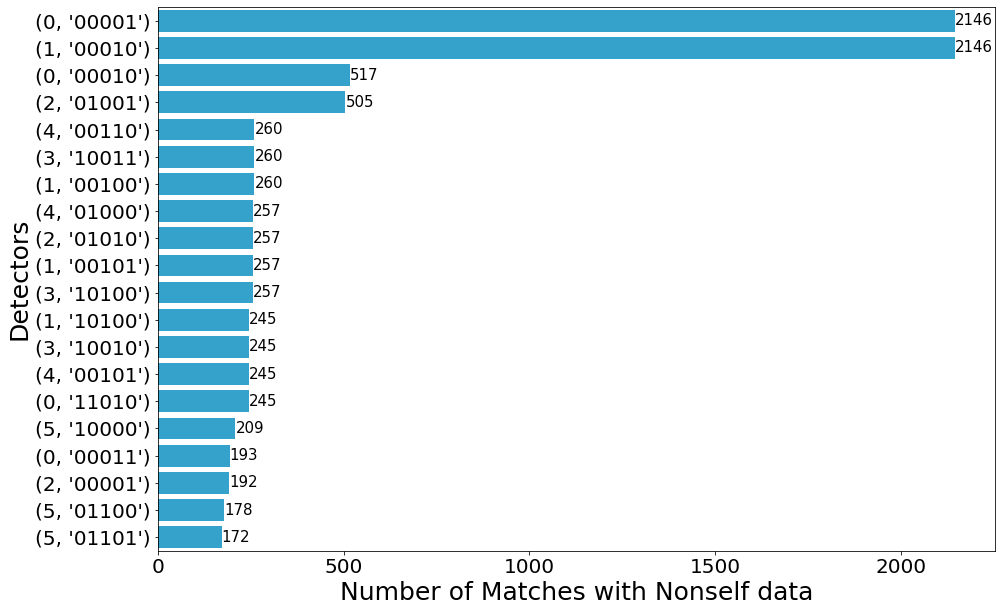
\includegraphics[width=0.8\textwidth, keepaspectratio]{img/matches_by_detector_rdz.png}
	\caption{Top 20 Detectors with most matches}
	\label{fig:ev_det_match}
\end{figure}

The bar chart in Figure \ref{fig:ev_det_match} displays the amount of nonself data that were matched by the top 20 detectors. This chart provides the analyst a better understanding of which are the most common and relevant patterns that were found by the algorithm.

By looking at the chart from Figure \ref{fig:ev_det_match}, one can easily see that the first two detectors match the same amount of nonself data. Besides that, their patterns seem to overlap, since if they were placed next to each other, considering their position, the difference between the two is the leftmost bit on the first one and the rightmost bit on the second one. This raised the possibility of two or more detectors having detected the same pattern but, because of the fixed size of the R-chunk, they were separated. In order to verify this situation, the MCC rate was computed for each pair of detectors. In the case of a pair being perfectly correlated, we could infer that they had matched the exact same nonself data, thus, they could be seen as the same pattern stored in different detectors. The idea was to agglutinate such pairs in order to have more robust patterns. For example, the first two detectors from Figure \ref{fig:ev_det_match} became a single 6-bit string detector, starting in position 0, with the bits \textit{000010}. After identifying and agglutinating all the identified cases, the total amount of detectors became 49.

\begin{figure}[]
	\centering
	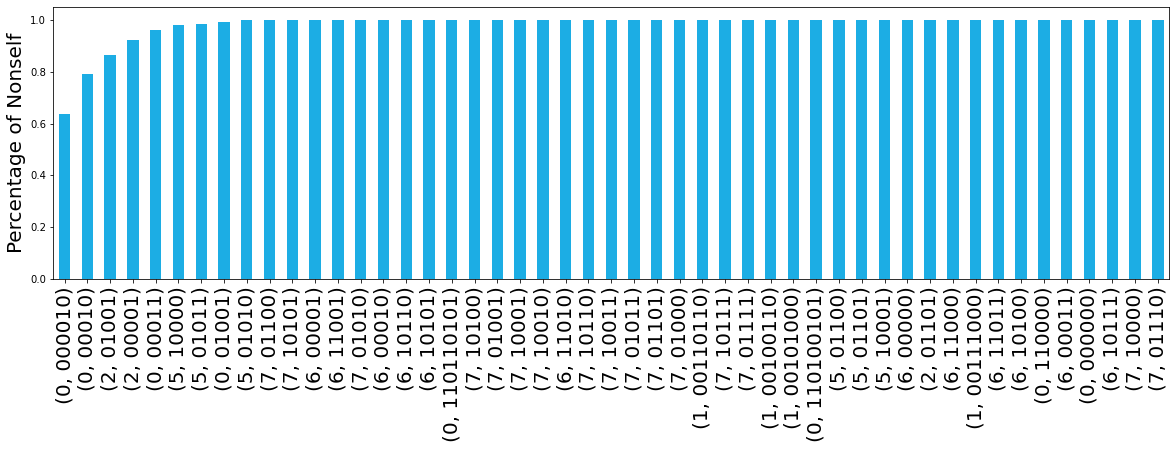
\includegraphics[width=\textwidth, keepaspectratio]{img/det_coverage.png}
	\caption{Coverage of Nonself data matched by detectors}
	\label{fig:ev_det_cov}
\end{figure}

Another aspect that need to be considered is the fact that the sum of matches is still greater than the amount of property violation cases in the dataset. Figure \ref{fig:ev_det_cov} depicts the percentage of nonself data covered with the addition of the detectors one by one, sorted by relevance. From the chart, we see that only 9 detectors are capable of detecting all the anomalous behavior of the system. 

This information raises a relevant fact. The set of nonself data matched by some detectors may comprise the entire set of other detectors with less matches. Another way of looking at it is to think that the patterns found by some detectors are part, or even specializations, of greater patterns of nonself data. Figure \ref{fig:ev_pattern_spec} attempts to illustrate this concept. By analyzing the detectors, we saw that all of the patterns matched by the detector \textit{(1,'00111000')} were also matched by \textit{(0,'00011')}. Moreover, the detector \textit{(0,'00011')} also matched all the nonself data matched by \textit{(1,'001101100')}. Therefore, it is possible to state that the pattern \textit{(0,'00011')} is specialized into the two other patterns, meaning that the bigger pattern can happen under two different circumstances, accounted by the two other patterns.

\begin{figure}[]
	\centering
	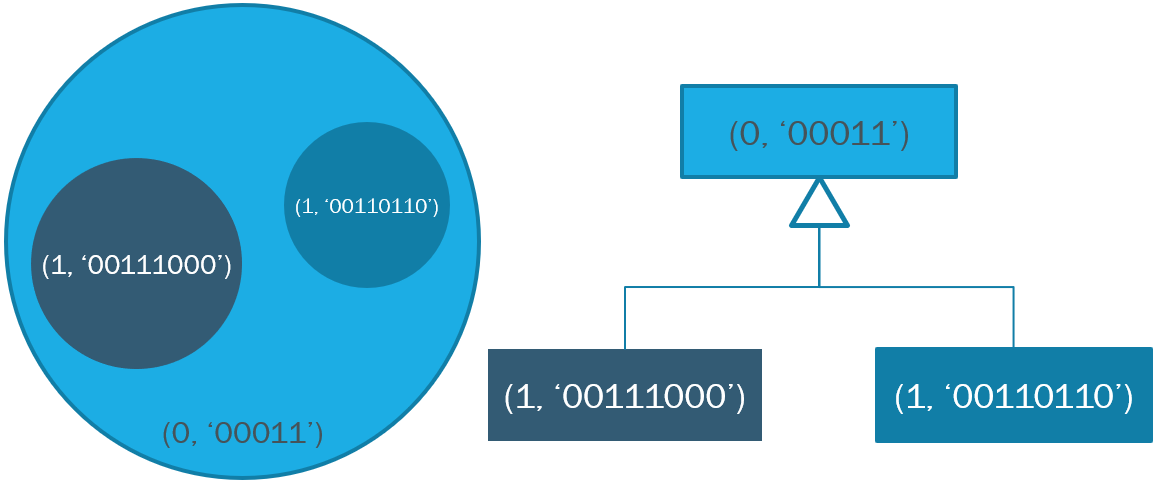
\includegraphics[width=0.7\textwidth, keepaspectratio]{img/pattern_specialization.png}
	\caption{Specialization of Patterns}
	\label{fig:ev_pattern_spec}
\end{figure}

Figure \ref{fig:ev_pattern_spec_reverse_mapping} shows the reverse mapping of the highlighted patterns. The detectors were placed in their respective positions, side by side, and the relevat rows from Table \ref{tab:pos_features} were brought for a better understanding of the patterns found. The leftmost pattern is the one that is specialized in the other two. By the boolean values and the positions, we see that it is related to the violations that happen when the data transference from the sensor to the Central Node did not happen (signal 0 in position 1) and the battery ran out at some point during the trace (signal 1 in position 3). The observer in the middle share this same pattern, but specifies the cases when the battery ran out during the processing of the data (signal 1 in position 7). In the meanwhile, the righmost observer points to the scenarios when the battery ran out while the sensor was acquiring the patient's vital signs. In summary, this group of detectors indentified the cases where the violation happened because the data was not transfered due to the battery running out either during the collection or the processing of the data.


\begin{figure}[!h]
	\centering
	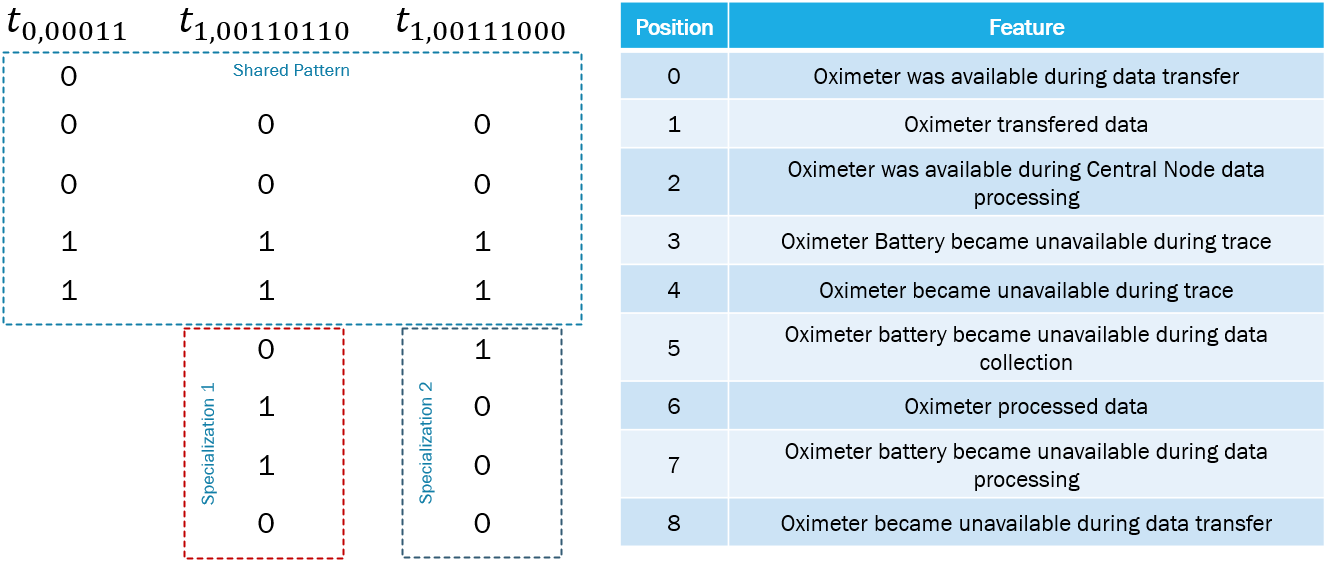
\includegraphics[width=\textwidth, keepaspectratio]{img/pattern_specialization_reverse_map.png}
	\caption{Reverse Mapping of the Specialized Patterns}
	\label{fig:ev_pattern_spec_reverse_mapping}
\end{figure}

This analysis should provide the CPS analyst with substantial information to address the situation. By looking at this specific scenario, it is possible to understand that the battery is key for the satisfaction of the property \textbf{P7}. This happens since the cell may run out during the collection or the processing of the data, making it impossible for the Central Node to process it within the time restriction. Therefore, it could be the case for the analyst to update de observer related to the property \textbf{P7}, so that it would consider this newly unveiled variability. Figure \ref{fig:ev_observer_fxd} illustrates the changes that could be made to the observer of the property \textbf{P7}, based on the Observer catalog from \cite{2022PSP}. A new state related to the battery being off would be created so that, if this component runs out after the data was acquired, then the error state would not be reached.

\begin{figure}[]
	\centering
	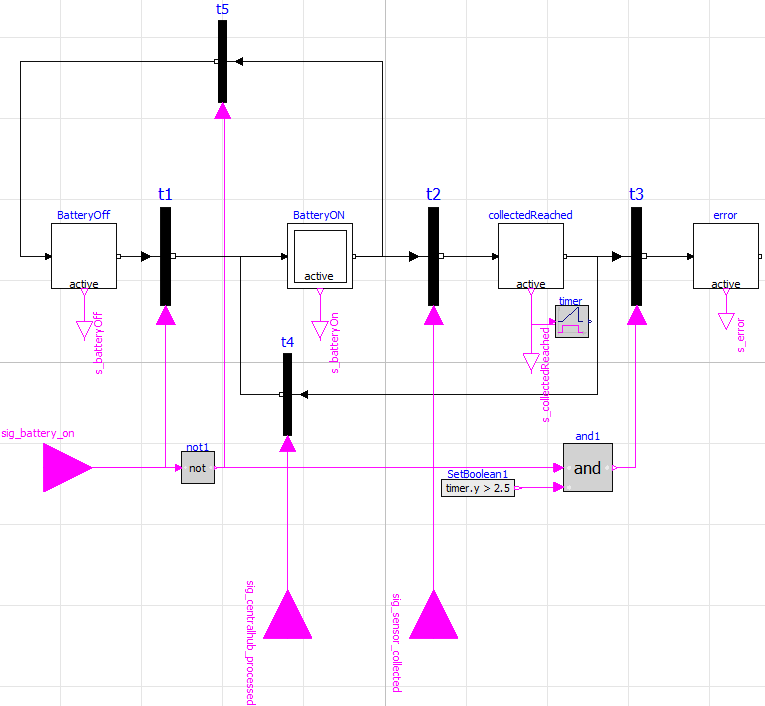
\includegraphics[width=0.7\textwidth, keepaspectratio]{img/observer_fxd.png}
	\caption{P7's Observer updated}
	\label{fig:ev_observer_fxd}
\end{figure}

Finally, the patterns and their specializations were all computed and are laid out in Figure \ref{fig:ev_sankey}. The Sankey chart helps us not only to understand the relationship amongst the detectors, but it also provides a visual aid for identifying the strength of the relation. In the figure, the most relevant detectors are placed on the left side of the pair, and their specialization are displayed in the right side. The strength of the relation can be seen in the line that connects them. The larger the line connecting two points is, the more nonself data are detected by the pair. Some relations are simple as the exemple from Figure \ref{fig:ev_pattern_spec}, but others can bring more complex structures, like the group formed by detector \textit{(5, '01011)}.

\begin{figure}[]
	\centering
	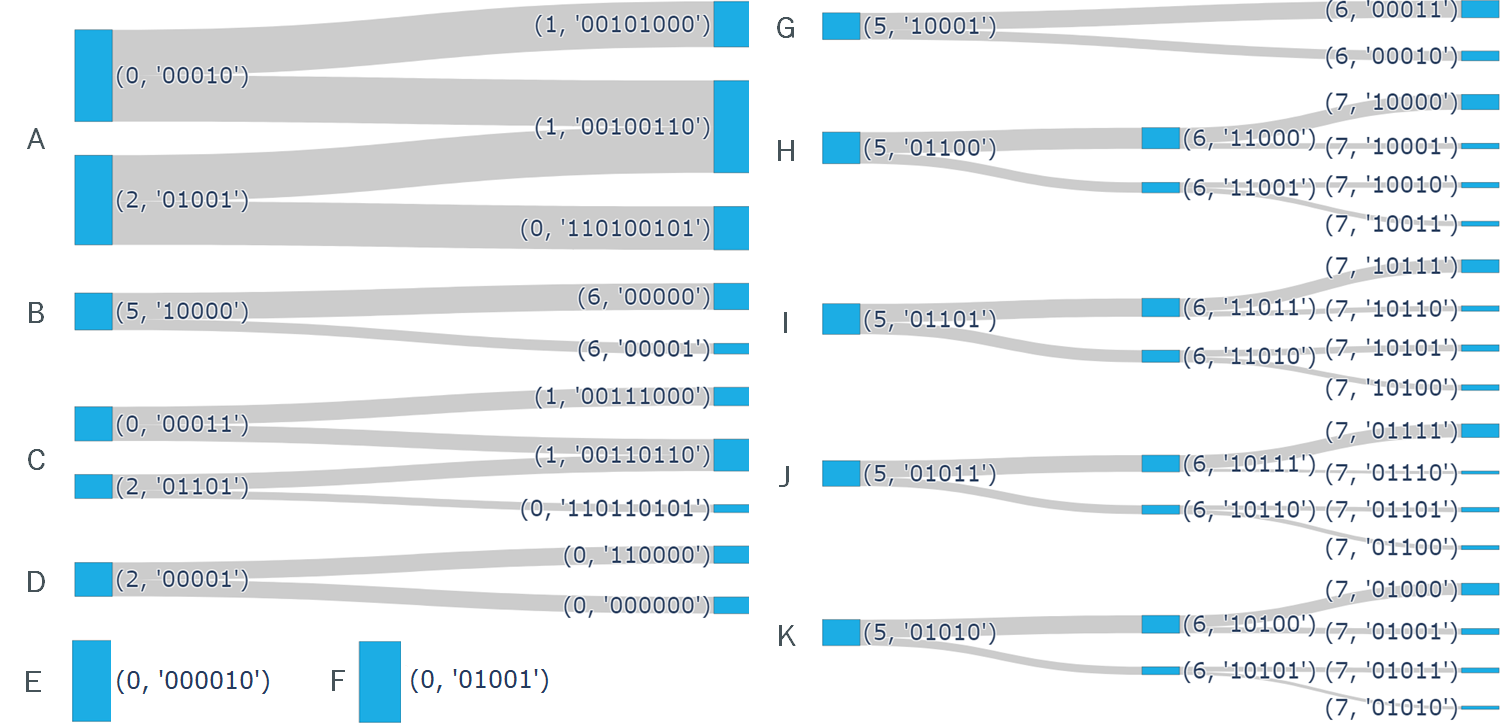
\includegraphics[width=\textwidth, keepaspectratio]{img/sankey3.png}
	\caption{Groups of Detectors identified based on the similarity of patterns}
	\label{fig:ev_sankey}
\end{figure}

Figure \ref{fig:pyramid} illustrates the overall process of finding relevant patterns. From the 229 detectors generated by the Negative Selection Algorithm, only 68 have matched with nonself data. From those, we concluded that some of them were actually the same pattern, splitted into two or more detectors due to the size limitation of the R-chunk, and thus, could be agglutinated. After merging them, the resultant 49 detectors were grouped into 11 clusters of patters with common behavior. These violation-related patterns found in the operation dataset account for the effectiveness of the approach in discovering patterns in data since the were shown to be relevant for the refinement of property \textbf{P7} runtime monitor.

\begin{figure}[!h]
	\centering
	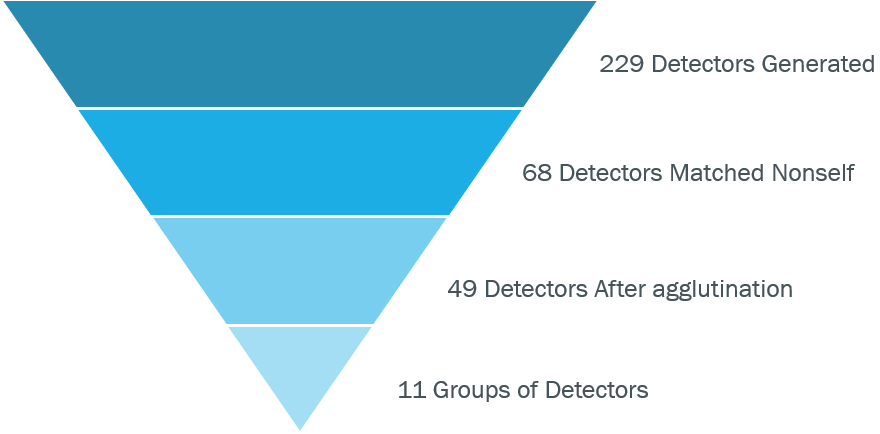
\includegraphics[width=0.5\textwidth, keepaspectratio]{img/detector_piramid.png}
	\caption{Number of Detectors at each step}
	\label{fig:pyramid}
\end{figure}

Table 
\ref{tab:patterns_detector_group} 
elaborates on the sankey chart. It provides more information on the pattern that was identified for each detector group, along with the respective percentage of nonself data matched within each set. A total of 63\% of the nonself set matched with the detector from Group E. From the description, we can see that it accounts for the cases when the sensor stopped responding, was too far away to transmit reliable data, or had some malfunctioning of sorts that may account for faults in runtime. Group A was the second in percentage of matches, accounting for near 21\% of the total of anomalous data. This group matches the cases in which the data was not transmitted due to the battery running out either during the data collection, processing or transfering. 

\begin{table}[]
	\centering
	\small
	\begin{tabular}{cccccc}
	\hline
	\makecell{Pattern \\Group}                           & Detector 1    & Detector 2       & Detector 3                       & Pattern Description                                                                      & \makecell{Percentage of \\Nonself matched} \\ \hline
	\multicolumn{1}{c|}{\multirow{3}{*}{A}} & (0, '00010')  & (1,'00101000')   & \multicolumn{1}{c|}{}            & \multicolumn{1}{c|}{\makecell{Lack of battery \\during data collection}}                            & 7,61\%                        \\ \cline{2-6} 
	\multicolumn{1}{c|}{}                   & (0, '00010')  & (1,'00100110')   & \multicolumn{1}{c|}{(2,'01001')} & \multicolumn{1}{c|}{\makecell{Lack of battery \\during data processing}}                              & 7,70\%                        \\ \cline{2-6} 
	\multicolumn{1}{c|}{}                   & (2,'01001')   & (0,'110100101')  & \multicolumn{1}{c|}{}            & \multicolumn{1}{c|}{\makecell{Lack of battery \\during data transfering}}                             & 7,26\%                        \\ \hline
	\multicolumn{1}{c|}{\multirow{2}{*}{B}} & (5,'100000')  & (6,'00000')      & \multicolumn{1}{c|}{}            & \multicolumn{1}{c|}{\multirow{2}{*}{\makecell{Lack of battery \\during data collection}}}             & 4,41\%                        \\ \cline{2-4} \cline{6-6} 
	\multicolumn{1}{c|}{}                   & (5,'100000')  & (6,'00001')      & \multicolumn{1}{c|}{}            & \multicolumn{1}{c|}{}                                                                    & 1,78\%                        \\ \hline
	\multicolumn{1}{c|}{\multirow{3}{*}{C}} & (0,'00011')   & (1,'00111000')   & \multicolumn{1}{c|}{}            & \multicolumn{1}{c|}{\makecell{Lack of battery \\during data collection}}                              & 3,05\%                        \\ \cline{2-6} 
	\multicolumn{1}{c|}{}                   & (0,'00011')   & (1,00110110')    & \multicolumn{1}{c|}{(2,'01101')} & \multicolumn{1}{c|}{\makecell{Lack of battery \\during data processing}}                              & 2,67\%                        \\ \cline{2-6} 
	\multicolumn{1}{c|}{}                   & (2,'01101')   & (0,'110110101')  & \multicolumn{1}{c|}{}            & \multicolumn{1}{c|}{\makecell{Sensor was off \\during transfer}}                                      & 1,33\%                        \\ \hline
	\multicolumn{1}{c|}{\multirow{2}{*}{D}} & (2,'00001')   & (0,'110000')     & \multicolumn{1}{c|}{}            & \multicolumn{1}{c|}{\multirow{2}{*}{\makecell{Sensor was off during \\Central Node processing}}} & 2,90\%                        \\ \cline{2-4} \cline{6-6} 
	\multicolumn{1}{c|}{}                   & (2,'00001')   & (0,'000000')     & \multicolumn{1}{c|}{}            & \multicolumn{1}{c|}{}                                                                    & 2,79\%                        \\ \hline
	\multicolumn{1}{c|}{E}                  & (0,'000010')  &                  & \multicolumn{1}{c|}{}            & \multicolumn{1}{c|}{\makecell{Sensor was off \\at some point}}                                        & 63,59\%                       \\ \hline
	\multicolumn{1}{c|}{F}                  & (0,'01001')   &                  & \multicolumn{1}{c|}{}            & \multicolumn{1}{c|}{\makecell{Sensor was off during \\Central Node processing}}                  & 0,68\%                        \\ \hline
	\multicolumn{1}{c|}{\multirow{2}{*}{G}} & (5,'10001')   & (6,'00011')      & \multicolumn{1}{c|}{}            & \multicolumn{1}{c|}{\multirow{2}{*}{\makecell{Lack of battery \\during data collection}}}             & 2,84\%                        \\ \cline{2-4} \cline{6-6} 
	\multicolumn{1}{c|}{}                   & (5,'10001')   & (6,'00010')      & \multicolumn{1}{c|}{}            & \multicolumn{1}{c|}{}                                                                    & 1,63\%                        \\ \hline
	\multicolumn{1}{c|}{\multirow{4}{*}{H}} & (5,'01100')   & (6,'11000')      & \multicolumn{1}{c|}{(7,'10000')} & \multicolumn{1}{c|}{\multirow{4}{*}{\makecell{Lack of battery \\during data processing}}}             & 2,58\%                        \\ \cline{2-4} \cline{6-6} 
	\multicolumn{1}{c|}{}                   & (5,'01100')   & (6,'11000')      & \multicolumn{1}{c|}{(7,'10001')} & \multicolumn{1}{c|}{}                                                                    & 0,95\%                        \\ \cline{2-4} \cline{6-6} 
	\multicolumn{1}{c|}{}                   & (5,'01100')   & (6,'11001')      & \multicolumn{1}{c|}{(7,'10010')} & \multicolumn{1}{c|}{}                                                                    & 0,92\%                        \\ \cline{2-4} \cline{6-6} 
	\multicolumn{1}{c|}{}                   & (5,'01100')   & (6,'11001')      & \multicolumn{1}{c|}{(7,'10011')} & \multicolumn{1}{c|}{}                                                                    & 0,83\%                        \\ \hline
	\multicolumn{1}{c|}{\multirow{4}{*}{I}} & (5,'01101')   & (6,'11011')      & \multicolumn{1}{c|}{(7,'10111')} & \multicolumn{1}{c|}{\multirow{4}{*}{\makecell{Lack of battery \\during data processing}}}             & 2,16\%                        \\ \cline{2-4} \cline{6-6} 
	\multicolumn{1}{c|}{}                   & (5,'01101')   & (6,'11011')      & \multicolumn{1}{c|}{(7,'10110')} & \multicolumn{1}{c|}{}                                                                    & 0,89\%                        \\ \cline{2-4} \cline{6-6} 
	\multicolumn{1}{c|}{}                   & (5,'01101')   & (6,'11010')      & \multicolumn{1}{c|}{(7,'10101')} & \multicolumn{1}{c|}{}                                                                    & 1,10\%                        \\ \cline{2-4} \cline{6-6} 
	\multicolumn{1}{c|}{}                   & (5,'01101')   & (6,'11010')      & \multicolumn{1}{c|}{(7,'10100')} & \multicolumn{1}{c|}{}                                                                    & 0,95\%                        \\ \hline
	\multicolumn{1}{c|}{\multirow{4}{*}{J}} & (5,'01011')   & (6,'10111')      & \multicolumn{1}{c|}{(7,'01111')} & \multicolumn{1}{c|}{\multirow{4}{*}{\makecell{Lack of battery \\during data transfering}}}            & 2,28\%                        \\ \cline{2-4} \cline{6-6} 
	\multicolumn{1}{c|}{}                   & (5,'01011')   & (6,'10111')      & \multicolumn{1}{c|}{(7,'01110')} & \multicolumn{1}{c|}{}                                                                    & 0,50\%                        \\ \cline{2-4} \cline{6-6} 
	\multicolumn{1}{c|}{}                   & (5,'01011')   & (6,'10110')      & \multicolumn{1}{c|}{(7,'01101')} & \multicolumn{1}{c|}{}                                                                    & 0,77\%                        \\ \cline{2-4} \cline{6-6} 
	\multicolumn{1}{c|}{}                   & (5,'01011')   & (6,'10110')      & \multicolumn{1}{c|}{(7,'01100')} & \multicolumn{1}{c|}{}                                                                    & 0,71\%                        \\ \hline
	\multicolumn{1}{c|}{\multirow{4}{*}{K}} & (5,'01010')   & (6,'10100')      & \multicolumn{1}{c|}{(7,'01000')} & \multicolumn{1}{c|}{\multirow{4}{*}{\makecell{Lack of battery \\during data transfering}}}            & 1,99\%                        \\ \cline{2-4} \cline{6-6} 
	\multicolumn{1}{c|}{}                   & (5,'01010')   & (6,'10100')      & \multicolumn{1}{c|}{(7,'01001')} & \multicolumn{1}{c|}{}                                                                    & 1,01\%                        \\ \cline{2-4} \cline{6-6} 
	\multicolumn{1}{c|}{}                   & (5,'01010')   & (6,'10101')      & \multicolumn{1}{c|}{(7,'01011')} & \multicolumn{1}{c|}{}                                                                    & 0,80\%                        \\ \cline{2-4} \cline{6-6} 
	\multicolumn{1}{c|}{}                   & (5,'01010')   & (6,'10101')      & \multicolumn{1}{c|}{(7,'01010')} & \multicolumn{1}{c|}{}                                                                    & 0,53\%                        \\ \hline
	\end{tabular}
    \caption{Description of the patterns found in each Detector Group}
	\label{tab:patterns_detector_group}
\end{table}

\section{Discussion}

Even though there are several methods for verifying a system for assurance purposes, such as Model Checking or runtime verification, the structural, dynamic, and organizational complexities of Cyber-Physical systems may become an impediment in this process, both in modeling and in defining the set of properties that will be assessed. The technique proposed in this paper seeks to fill this gap by utilizing well-studied frameworks for modeling the complex link between the discrete-time behavior of software components and the continuous-time acausal equations that govern the physical processes of such systems. Furthermore, the simulated data analysis enables the detection of patterns in data that could not have been accounted for when the system properties were initially elicited. Thus, our technique provides a better understanding of the context in which the CPS will be introduced, allowing the verification process to be enhanced.

Our technique's quantitative evaluation yielded satisfactory results. The use of the Negative Selection Algorithm resulted in performance that was quite close to that of other proeminent Machine Learning algorithms, including those specialized in anomaly detection. The NSA gave a low \textit{False Positive} rate in the presence of unseen data, meaning that no mistakes that could harm the proposed technique occurred. Aside from that, the examination of the patterns discovered by the detectors was also quite good. We were able to select 49 detectors from the 229 produced detectors that were truly important for characterizing property violations that may occur at runtime. Those detectors were also distributed into 11 clusters based on the similarity of the discovered patterns, further assisting the software analyst by displaying the components that are closely connected to the source of the anomalous behavior.


\section{Threats to validity}

\begin{itemize}
    \item \textbf{Construct validity:} We relied on a documented case study  (BSN) and its publicly accessible data to ensure that we present a valid and sound input for our evaluation. The specification of the system, in the form of a CGM, as well as the properties derived from it and the observers utilized were all taken from literature. Besides that, the patient profiles were generated based on a randomized process in order to minimize as much as possible bias in the data. However, in spite of our efforts to avoid generating inaccurate data, we were not able to guarantee that the created data represents accurately a real-world circumstance. Further research is required to validate such representation.
    
    \item \textbf{Internal validity:} Our evaluation relies significantly on the BSN prototype implemented in Modelica, since the patterns discovered are only as good as the dataset used to find them. Therefore, a correct abstraction of the behavior of the BSN into a model for simulation is paramount. The model must account for as much variability as possibile, according to what will be faced during the execution of the CPS. Nevertheless, it is of our understanding that this is not an easy task. Even with the right tools and state-of-the-art framework, the expert's knowledge of the system is highly required, since several aspects of the system are specific for the medical domain. Besides that, differential equations are used to model the behavior of the physical components, which would also need a more specialized opinion. As stated by Baier and Katoen \cite{2008PrinciplesModelChecking}, "Any verification using model-based techniques is only as good as the model of the system."
    
    Moreover, the choice for the binary version of the Negative Selection Algorithm also comes with its disadivantages. Even though modeling the behavior of the CPS as boolean features allows for simplicity and the reverse mapping of binary detectors provide a great level of interpretability, the Binary Negative Selection (BNSA) is well-known for its performance and completeness issues. D'haeseleer et al. \cite{NSADetGen1996} pointed out that the generation of binary detectors is a very time-conusming task, that rises exponentially with the size of the self-set. They also state the possible existence of "holes", which are strings for which is impossible to generate valid detectors. This would account for property violation patterns impossible to be unveiled, thus, decreasing the efficiency of our approach. Finally, they also say that an accurate and stable definition of self is key for the success of the BNSA, which is not always the case due to the dynamic complexities of CPS.
	
	\item \textbf{External validity:} Even though our technique is not domain specific, we understand the evaluation's limitations because it was applied in single example of the medical field. Further study of the technique is required to determine the approach's true usefulness for generalization goals. To assess the technique's real applicability for purposes of generalization, more examination of the technique must be done.
    
\end{itemize}